\documentclass[12pt,a4paper]{article}

% Balíčky pro kódování, fonty a jazyk
\usepackage[utf8]{inputenc}
\usepackage[T1]{fontenc}
\usepackage[czech]{babel}


\usepackage{float} % lepsi umistovani obrazku (H)
\usepackage{xparse} % lepsi commandy s optional params
\usepackage{hyperref} % vkladani hypertextovych odkazu
\usepackage{enumitem} % lepsi enumerate a descrition and so on
\usepackage{wrapfig} % obrazky obtekané textem
\usepackage{longtable} % tabulky na více stran
\usepackage{latexsym} % symboly


% Balíčky pro lepší formátování textu
\usepackage{microtype} % Vylepšení typografie
\usepackage{lipsum}    % Generování náhodného textu

% Balíčky pro práci s obrázky
\usepackage{graphicx}
\graphicspath{{images/}} % Cesta k adresáři s obrázky

% Balíček pro lepší práci s odkazy
\usepackage{hyperref}
\hypersetup{
    colorlinks=false, % vypne barevné odkazy
    pdfborder={0 0 0} % nastaví hranice odkazů na 0, aby se nezobrazovaly rámečky
}

% Nastavení geometrie stránky
\usepackage{geometry}
\geometry{
 a4paper,
 total={170mm,257mm},
 left=20mm,
 top=20mm,
}
% odsazení odstavců
\setlength{\parskip}{1em}
\setlength{\parindent}{0pt} % Vypne odsazení odstavců

% nastavení minted
\immediate\write18{echo $ROAD > .ROAD.tex}
\immediate\write18{echo $ROAD "tohle je ten nejhorší hack co jsem kdy udělal"} 
\input{.ROAD}
\usepackage[outputdir=\ROAD]{minted} %
\setminted{fontsize=\small, baselinestretch=1, frame=lines, framesep=8pt, linenos, breaklines}
%\usemintedstyle{murphy}


% Údaje pro titulní stranu
\title{Příručka pro vývoj API}
\author{Martin Korotwitschka}
%\date{\today}

% Začátek dokumentu
\begin{document}

\maketitle % Vytvoří titulní stranu

\begin{abstract}
    Tento dokument slouží jako neformální příručka pro vývoj API poskytující praktické informace a tipy pro vývojáře.
\end{abstract}

\tableofcontents % Vytvoří obsah na základě sekcí a podsekcí

\newpage


\section{Úvod}\label{sec:api-goal}

Je důležité si uvědomit, že kvalitní návrh a pečlivá definice klíčových mechanismů projektu jsou základem pro úspěch jakéhokoli API. Tyto počáteční kroky určují strukturu a funkčnost API, které slouží jako zprostředkovatel mezi uživateli a systémem. Při návrhu API je třeba pečlivě zvážit, jaké typy operací a datových interakcí bude potřeba podporovat, aby byly splněny specifické potřeby aplikace.

\section{Jak na návrh}\label{sec:api-how}

Na samém začátku je klíčové pečlivě navrhnout, jaké funkce bude naše API nabízet a jak celkově bude aplikace fungovat. Musíme přesně specifikovat, jakou funkcionalitu od API očekáváme, protože na základě těchto požadavků definujeme koncové body. Tyto základní funkční požadavky následně použijeme jako výchozí bod pro návrh API a všech věcí okolo.

Tento obecný přístup k návrhu API bude nyní demonstrováno na příkladu naší hry, kde ukážeme praktické aplikace teoretických principů. Následovat bude detailní pohled na návrh a funkční požadavky specifické pro naši hru.

\section{Návrh API pro hru}\label{sec:api-design}

Jako první se může provést tzv. analýza funkčních požadavků. Ta v našem případě zahrnuje definici funkcí a takhle nějak by mohly vypadat:

\subsection{Funkční požadavky}

\subsubsection*{Požadavky, které byly vyčleněny primárně ze strany backoffice}

\begin{enumerate}[label=\textbf{F\arabic*}:, leftmargin=*, align=left]
    \item \textbf{CRUD operace} -- Nad základními objekty, se kterými se bude často pracovat, a upravovat pomocí endpointů. Těmito objekty jsou \texttt{akce, efekty, předměty, charaktery a jejich vlastnosti, dobrodružství, kampaň, obchody, nepřátelé, překážky, lokace} a \texttt{části lokace}
    \item \textbf{Filtrování} -- Možnost vyhledat objekty podle vstupních parametrů u koncových bodů, které poskytují seznam objektů.
    \item \textbf{Lazy load} -- Způsob načítání dat, který umožňuje vracet pouze daný objekt bez jeho závislostí, případně vrácení pouze těch závislostí, které se určí. Výsledkem je rychlejší zpracování a menší objem přesunutých dat, když uživatel tyto závislosti nepotřebuje. Namísto objektu se tedy vrátí jen jeho identifikátor.
    \item \textbf{Stránkování} -- Další způsob předávání dat, který umožní jejich postupné zpracování, což vede ke zkrácení času potřebného k vyhodnocení požadavku jak v API tak ve zobrazovací části.
    \item \textbf{Caching} -- Již jednou zpracovaná data z databáze není třeba znovu získávat z databáze, pokud nedošlo ke změně. Tato funkcionalita umožní násobně rychlejší odezvu pro opakované získávání stejných dat.
    \item \textbf{Administrátorská práva} -- Ne všichni mohou mít přístup pro úpravu dat v databázi. Díky administrátorským přihlašovacím údajům a následnému tokenu se budou moci upravovat a vkládat data do databáze pouze s odpovídajícím ověřením.
    \item \textbf{Validace} -- Data vkládaná do databáze budou validována a případně vrátí chybovou hlášku, podle které bude možno snadno identifikovat chybu vstupních dat a následně ji opravit.
\end{enumerate}


\subsubsection*{Požadavky primárně ze strany uživatelského prostředí}

\begin{enumerate}[label=\textbf{F\arabic*}:, leftmargin=*, align=left]
    \item \textbf{Získávání objektů} -- Bude umožněno získávat jakékoliv objekty, které neobsahují herní data či jiné citlivé informace, přímo z databáze.
    \item \textbf{Podpora herního průběhu} -- Uživatel bude moci projít celým soubojem a interagovat s entitami v něm za pomocí řady validovaných a přehledně uspořádaných koncových bodů.
    \item \textbf{Zamezení zneužití} -- Postup operací v herním průběhu bude kontrolován tak, aby se zamezilo případnému zneužití nebo obcházení pravidel hry.
    \item \textbf{Přihlášení} -- Uživatel se bude moci přihlásit a získat token pro ověření v dalších požadavcích.
    \item \textbf{Herní data} -- Uživatel bude mít pod svým účtem uložený postup hry a bude moci pokračovat tam, kde skončil. Dále bude mít možnost vytvářet nové postavy pro kampaně a také nová dobrodružství.
    \item \textbf{Validace} -- Obsah vstupních dat bude validován a případně vrátí smysluplnou chybovou hlášku.
    \item \textbf{Obrázky} -- Bude možné získat obrázek z url adresy přiložené k objektu, případně v požadavku specifikovat jeho velikost.
\end{enumerate}


\subsection{Nefunkční požadavky}
Dále je důležité vyhradit si nefunkční požadavky. Jejich vznik je stejný jako požadavky funkční, byly sestrojovány postupně s vývojem na základě zkušeností a požadavků ostatních členů týmu.


\begin{enumerate}[label=\textbf{F\arabic*}:, leftmargin=*, align=left]
    \item \textbf{Rozdělení API na dvě části} -- Z důvodu spolupráce na API s jinými členy týmu, především herním systémem, který pro svůj chod využívá stejných modelů, bylo rozhodnuto, že herní logika i mapování bude v jednom projektu. Tomu tedy musí být přizpůsobena i spolupráce a podpůrné technologie.
    \item \textbf{Dokumentace} API bude zdokumentováno za pomocí OpenAPI a pro vizuální zobrazení koncových bodů bude použit Swagger, který zároveň poslouží jako skvělé ladící rozhraní.
    \item \textbf{Hosting} API bude stejně jako ostatní části projektu hostováno na veřejných serverech.
    \item \textbf{Přehlednost} Koncové body API by měly být samopopisující a snadno pochopitelné.
    \item \textbf{Standardizovanost} API se bude držet ověřených dobrých praktik z praxe a bude udržovat jednotnost a standardizovanost.
\end{enumerate}


\section{Výběr technologií}\label{sec:api-tech}

Návrh API zahrnuje řadu rozhodnutí, od volby architektonického stylu až po výběr konkrétních technologií a frameworků. Každý z těchto výběrů by měl být motivován specifickými potřebami vašeho projektu, včetně typů operací, které bude API podporovat, očekávané zátěže, bezpečnostních požadavků a dalších faktorů.

\subsection{Volba Architektury API}
\subsubsection*{REST}
\textbf{Definice:} REST (Representational State Transfer) je architektura založená na standardních HTTP metodách, která využívá jednoduché URL pro přístup k zdrojům a HTTP metody jako GET, POST, PUT a DELETE pro operace nad nimi.

\textbf{Usecase:} REST je ideální pro většinu webových aplikací, které vyžadují škálovatelnost, jednoduchost a snadnou integraci s webovými prohlížeči. REST je široce používán pro veřejné API, například Google Maps API nebo Facebook Graph API.

\subsubsection*{GraphQL}
\textbf{Definice:} GraphQL je jazyk dotazů pro API vyvinutý Facebookem, který umožňuje klientům specifikovat přesně, jaké data potřebují, což může redukovat množství dat přenesených přes síť.

\textbf{Usecase:} GraphQL je vhodné pro aplikace, které potřebují velkou flexibilitu v tom, jak a jaká data si mohou vyžádat, například mobilní aplikace, které potřebují minimalizovat množství dat přenášených přes mobilní sítě. Příkladem může být GitHub GraphQL API, které umožňuje uživatelům efektivněji získávat specifické informace o repozitářích, uživatelích atd.

\subsection{Výběr Frameworku}
\subsubsection*{Node.js s Express.js}
\textbf{Framework} Express.js je minimalistický a flexibilní Node.js web application framework, který poskytuje robustní soubor funkcí pro webové a mobilní aplikace.

\textbf{Usecase:} Express je často používán pro stavbu RESTful API díky své rychlosti a efektivitě. Je vhodný pro situace, kdy potřebujete rychle vyvíjet a iterovat, jako jsou startupy a nové produkty.

\subsubsection*{Spring Boot (Java)}
\textbf{Framework} Spring Boot umožňuje snadné vytvoření stojatých, produkčních aplikací na bázi Springu s minimem konfigurace.

\textbf{Usecase:} Spring Boot je vhodný pro komplexní podnikové aplikace, které vyžadují robustní bezpečnostní funkce, integrace s databázemi a podporu pro mikroslužby. Například Netflix používá Spring Boot ve své mikroslužbové architektuře.

\subsubsection*{Django (Python)}
\textbf{Framework} Django je vysokoúrovňový Python web framework, který podporuje rychlý vývoj a čistý, pragmatický design.

\textbf{Usecase:} Django je ideální pro rychlý vývoj aplikací s integrovanou podporou pro správu uživatelů, bezpečnost a databázové migrace, což ho činí vhodným pro webové aplikace a API s rychlým časovým horizontem k uvedení na trh.

\subsubsection*{ASP.NET Core}
\textbf{Framework:} ASP.NET Core je křížově platformní framework pro vývoj internetových aplikací od Microsoftu.

\textbf{Usecase:} ASP.NET Core je oblíbený v podnikových prostředích pro jeho výkon, bezpečnost a podporu pro vývoj v C\#, což usnadňuje integraci s jinými .NET aplikacemi a službami.

\subsection*{Závěr}
Výběr mezi REST a GraphQL by měl být založen na požadavcích vaší aplikace na komunikaci dat, zatímco výběr frameworku by měl odpovídat vašim technickým preferencím, očekávané škále a typu aplikace. Každý z těchto frameworků nabízí jedinečné výhody pro různé typy projektů a scénáře použití.
\chapter{Implementace}\label{chap:implementation}

\section{Implementace API}\label{sec:impl:api}
Implementace původně probíhala ve \gls{framework}u FastAPI \sectionref{sec:api_technologies:fast}, ale po zjištění složitosti ORM při použití Python knihovny SQL Alchemy bylo doporučeno jedním z řešitelů (P. Mikula), použít raději Javu a její \gls{framework} Spring Boot, za použití knihoven jako je JPA, Lombok, Jackson a jiných. Tato změna nebyla obtížná, jelikož vývoj byl teprve ve velice rané fázi vývoje. Taktéž Spring Boot byl jeden z kandidátů.

Nyní budou popsány nejdůležitější knihovny \gls{framework}u Spring Boot, které byly použity při implementaci \gls{api}.


\subsection{Knihovny Spring Boot}\label{sec:impl:spring}
% TODO nějaký lepší název nebo něco

Tyto knihovny jsou základním stavebním kamenem jak pro samotné koncové body tak pro \gls{orm}. Na obrázku \ref{fig:JPA} máme vizuální schéma toho, jak tyto knihovny spolu fungují.

\begin{figure}[ht!]
    \centering
    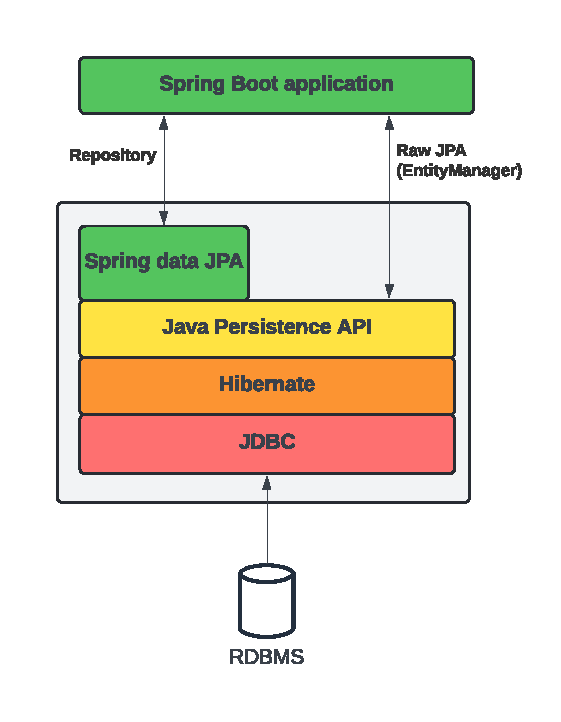
\includegraphics[width=0.5\textwidth]{figures/impl/API Implementation - JPA.pdf}
    \caption{Struktura Spring Boot Data JPA aplikace}
    \label{fig:JPA}
\end{figure}

\subsubsection*{Spring Data JPA} \label{sec:impl:spring:data:jpa}
JPA neboli Java Persistence API je jedna ze součástí Spring Data Family, která umožňuje jednoduché implementování \textbf{repozitářů} založených na JPA a signifikantně zjednodušuje implementaci datové vrstvy aplikace. Umožňuje používat základní SQL požadavky a ORM bez námahy vytvoření vlastních požadavků. V ukázce na výpisu \ref{code:JPA_repo} je vidět implementace repozitáře pro entitu \textit{Enemy}. Zde jsou již naimplementované základní metody jako \textit{save}, \textit{findAll}, a je zde navíc metoda \textit{findAllByLocationId} s vlastním SQL dotazem.

\begin{listing}[ht!]
    \inputminted[]{Java}{resources/code/impl/EnemyRepo.java}
    \caption{Ukázka JPA repozitáře}
    \label{code:JPA_repo}
\end{listing}

\subsubsection*{JPA}
Spring Data JPA používá několik dalších knihoven a dalo by se říci, že to je jakýsi zprostředkovatel nad \textbf{JPA}. JPA zajišťuje objektově relační mapování (\gls{orm}), což usnadňuje práci s ukládáním objektů do databáze a naopak.

Základním objektem v JPA je \textit{Entita}. Ta reprezentuje objekt v databázi, který je poté namapován na jednotlivé vlastnosti třídy \coderef{code:jpa_entity}. Třídu označíme jako entitu pomocí anotace \textit{@Entity} a poté pomocí \texttt{@Table} můžeme upřesnit jméno tabulky, schéma databáze a jiné atributy. Za pomoci anotace \textit{@Id} označíme primární klíč a nebo pomocí \texttt{@EmbeddedId} označíme složený primární klíč. Atributy třídy označíme pomocí \texttt{@Column} kdy ve výchozím stavu atribut může nabývat prázdné hodnoty a sloupec v databázi se jmenuje stejně jako atribut. Relace se mapují pomocí jedné z anotací \texttt{@OneToOne}, \texttt{@OneToMany}, \texttt{@ManyToOne} nebo \texttt{@ManyToMany} podle toho, jakou relaci potřebujeme. V této implementaci probíhal nejdříve návrh databáze, takže jsme používali pouze \texttt{1:N} relace abychom se vyhnuli cyklickým závislostem, protože vazební \texttt{M:N} tabulky již byly v databázi.

\subsubsection*{Hibernate}\label{sec:impl:hibernate}
Jedna z konkrétních implementací JPA je Hibernate. Za pomocí výše zmíněných anotací nebo XML \sectionref{sec:formats:xml} schématu si udržuje schéma databáze a stav objektů, udržuje tedy data perzistentní. Díky schématu databáze Hibernate ví, jak se mají data z databázových tabulek transformovat do objektů a naopak. \cite[]{enwiki:1217225259}

\subsubsection*{JDBC}\label{sec:impl:jdbc}
Neboli Java Database Connectivity je API pro přístup k databázi. Poskytuje metody pro dotazování se na na databázi pomocí \gls{sql} a umožňuje zpracovávat výsledky dotazů.

\begin{listing}[ht!]
    \inputminted[breaklines]{Java}{resources/code/impl/EnemyDTO.java}
    \caption{Příklad entity v JPA}
    \label{code:jpa_entity}
\end{listing}


\subsection{Jiné použité knihovny} %%TODO reformat nadpis aaaaaa
V této kapitole budou popsány knihovny, které nejsou součástí Spring Bootu, ale byly ve větší míře použity při implementaci API.

\subsubsection*{Lombok}\label{sec:impl:lombok}
Lombok je knihovna, která za pomocí anotací automaticky generuje základní repetetivní kódy jako jsou gettery a settery, konstruktory a jiné, což je pro vývojáře velice vítané.

První možností této knihovny jsou anotace \texttt{@Getter} a \texttt{@Setter}, které automaticky vygenerují \textbf{gettery} nebo \textbf{settery} s příslušnými modifikátory přístupu pro daný atribut \coderef{code:lombok:getters}. Tato anotace lze použít i nad celou třídou a automaticky vygeneruje kód pro všechny atributy. Vygenerované metody jsou ukázány na výpisu \ref{code:lombok:getters:generated}.

\begin{listing}[H]
    \begin{minted}[fontsize=\footnotesize]{Java}
        public class GetterSetterExample {
            @Getter private int age = 10;
            @Setter(AccessLevel.PROTECTED) private String name;
        }
     \end{minted}
    \caption{Použití anotací \texttt{@Getter} a \texttt{@Setter}}
    \label{code:lombok:getters}
\end{listing}

\begin{listing}[H]
    \begin{minted}[fontsize=\footnotesize]{Java}
        public class GetterSetterExample {
            private int age = 10;
            private String name;
            public int getAge() {
                return this.age;
            }
            protected void setName(String name) {
                this.name = name;
            }
        }
     \end{minted}
    \caption{vygenerovaný kód za pomocí \texttt{@Getter} a \texttt{@Setter}}
    \label{code:lombok:getters:generated}
\end{listing}

Další důležité anotace se týkají konstruktorů. \texttt{@NoArgsConstructor} vygeneruje prázdný konstruktor, \texttt{@AllArgsConstructor} vygeneruje konstruktor se všemi atributy \coderef{code:lombok:constructor} a jako poslední anotace \texttt{@RequiredArgsConstructor} vygeneruje konstruktor s všemi atributy označenými jako \texttt{@NonNull}. Tato anotace se zapisuje nad třídu. \cite{lombok:constructor}

\begin{listing}[H]
    \begin{minted}[fontsize=\footnotesize]{Java}
        public class ConstrExample {
            private int age;
            private String name;

            ConstrExample(int age, String name) {
                this.age = age;
                this.name = name;
            }
        }
    \end{minted}
    \caption{Příklad kódu vygenerovaného pomocí \texttt{@AllArgsConstructor}}
    \label{code:lombok:constructor}
\end{listing}


Práci si je možné zjednodušit ještě více za pomocí anotace \texttt{@Data}, která vygeneruje výše zmíněné \texttt{@Getter, @Setter, @RequiredArgsConstructor} a navíc \texttt{@ToString} a \texttt{@EqualsAndHashCode}.\cite{lombok:data} Anotace \texttt{@ToString} vygeneruje metodu \texttt{toString()}, která objekt převede na textový řetězec, kde za pomoci různých parametrů můžeme upravovat, které atributy se budou vypisovat a jak. Další anotace, kterou \texttt{@Data} obsahuje, je \texttt{@EqualsAndHashCode}, která vygeneruje metody pro porovnávání objektů.

Za zmínku také stojí anotace \texttt{@Builder}, která vygeneruje interní třídu podle návrhového vzoru Builder\cite{refactoringGuru:builder}, jež slouží k vytváření objektů. \cite{lombok:builder}

\subsubsection*{Jackson}\label{sec:impl:jackson}
Tato knihovna slouží pro serializaci objektů do formátu JSON \chapterref{sec:formats:json} a naopak. S její pomocí bylo možné specifikovat, jak se budou jednotlivé objekty či atributy serializovat, například zde lze nastavit ignorování některých atributů nebo úplně vlastní serializace.

\subsubsection*{Swagger}\label{sec:impl:swagger}
Swagger je open-source dokumentační nástroj pro \gls{restful api} zahnutý přímo v knihovně Spring Boot, který umožňuje vývoj API skrz celý jeho životní cyklus od návrhu přes dokumentaci a testování po nasazení. Využívá specifikaci OpenAPI, pomocí které dokáže generovat dokumentaci, interakci, testy a další.\cite{swagger:about} Tohoto nástroje jsme hojně využívali zvlášť pro interakci s koncovými body pro testování.

Ve Spring Bootu je jeho použití velmi jednoduché, stačí zaznamenat závislosti do \texttt{pom.xml} a přidat Springdoc Swagger konfiguraci do hlavního konfiguračního souboru.

\subsection{Serializace}\label{sec:impl:serialization}
% todo oprav si tu vetu pls wtf is this
% V rámci vývoje byla vytvořena vlastní třída pro serializaci relačních objektů pomocí vlastní třídy 
% %\coderef{code:lazyFieldsSerializer} TODO odkaz v přiložených souborech jaký to je soubor JEBAT THIS SHIT
% na serializování mapovaných objektů. 
Pro serializaci \sectionref{sec:formats:deserialization} relačních objektů byla vytvořena třída \texttt{LazyFieldsSerializer}, která se stará o serializaci objektů, které jsou označeny jako \texttt{lazy}.
Upravená metoda \texttt{serialize} zde zkontroluje, zda je serializovaný objekt instancí proxy a pokud ano, zda je objekt nainicializován. To za nás řeší metoda \texttt{Hibernate.isInitialized}.
%\coderef{code:lazyFieldsSerializer}[, řádek 56]. TODO to stejné jako výše
Pokud je tedy objekt nainicializován, serializuje se a dále na se jeho atributech opět volá metoda \texttt{serialize}. Pokud není nainicializován a nejedná se o kolekci, tak se serializuje pouze jeho id aniž by se objekt nainicializoval celý.
%\coderef{code:lazyFieldsSerializer}[, řádek 60]. TODO to stejné jako výše
Pokud se jedná o kolekci, musí se jednat o \texttt{M:N} tabulku a serializují se tedy všechny atributy kromě relací.
%\coderef{code:lazyFieldsSerializer}[, funkce \texttt{writeFieldsWithoutLazy() }]. TODO to stejné jako výše 


\subsection{Lazy load}\label{sec:impl:lazyload}
Pro tento účel musela být vytvořena metoda pro postupnou inicializaci. Pro rekurzivní načítání relačních objektů byla vytvořena statická metoda \texttt{hibernateInitializeAll()}, která přijme objekt a rekurzivně načte všechny jeho relace.
% nějaký ref
Tato funkce za pomocí \texttt{Hibernate.initialize()} nejdříve nainicializuje vstupní objekt a poté rekurzivně prochází všechny jeho atributy, přičemž přeskakuje ty, které nemají jednu z relačních anotací. Funkce má taktéž podporu filtru pro samotný lazy load, když se jméno atributu shoduje s jakýmkoli slovem ve filtru, atribut se přeskočí v inicializování.


\subsection{Koncové body}\label{sec:impl:endpoints}
Hlavním výstupem této práce je seznam koncových bodů \figureref{fig:action:endpoint} , které je možné použít pro administrativní část i hraní hry. Jednotlivé přístupové body jsou rozděleny do tzv. kontrolérů. Jako příklad zde je kontrolér pro entitu \textit{Character} \coderef{code:characterController}.

Níže \figureref{fig:endpoint:general} je zobrazen obecný diagram komponent koncového bodu. Třída \texttt{Controller} zde představuje komponentu poskytující koncové body klientům. Po příchozím požadavku ho přeposílá třídě \texttt{Service}, která se stará o jeho vyhodnocení. Při kladném výsledku data předá zpět třídě \texttt{Controller}, která je výsledek pošle klientovi. Pokud je výsledek záporný, je zachycena výjimka a klientovi je vracena přímo.

\begin{figure}[ht!]
    \centering
    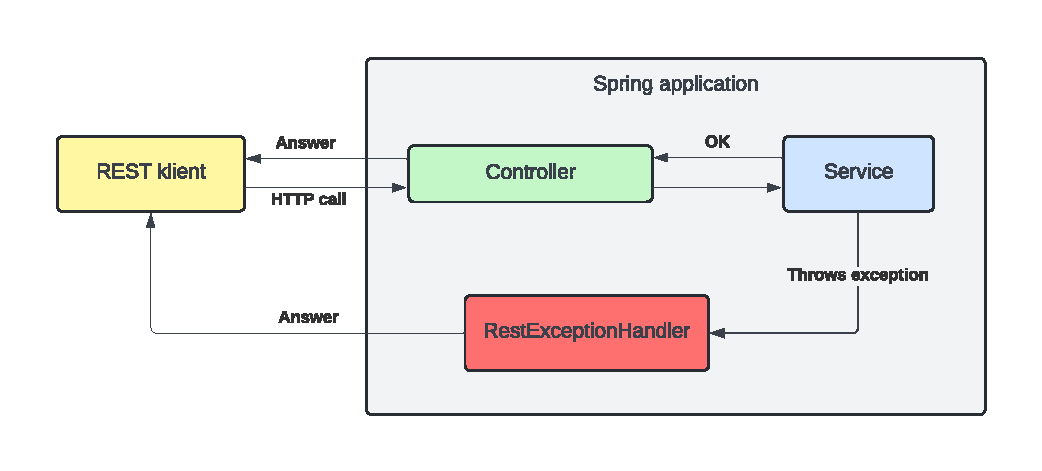
\includegraphics[width=0.9\textwidth]{figures/impl/API Implementation - endpoint.pdf}
    \caption{Obecný diagram koncového bodu}
    \label{fig:endpoint:general}
\end{figure}

Anotací \texttt{@RestController} určíme, že tato třída bude obsahovat koncové body. Dále pomocí anotace \texttt{@RequestMapping} zadáme cestu, pod kterou budou všechny koncové body v této třídě dostupné. A na závěr pomocí jednotlivých mapping anotací (\texttt{@GetMapping, @PutMapping @PostMapping @DeleteMapping}) určujeme, na jakou HTTP metodu má funkce reagovat.

Při mapování můžeme používat jak URI vzory pomocí regex výrazů (např \texttt{"/resources/*.png"}) tak i proměnné v URI (např \texttt{"/resources/{id}"}). Ten používáme třeba zde na výše zmíněném výpisu kontroléru postavy \coderef{code:characterController}[, řádek 9] pro získání jedné entity \textit{Character}. S tím se pojí anotace \texttt{@PathVariable}, která určuje, že vstupní parametr id bude brán z URI a bude se jednat o datový typ \texttt{int}.

Jako další můžeme používat tzv. \textit{query} parametry, které je možné získat získat za pomocí anotace \texttt{@RequestParam}, kde se může předem určit, zda je parametr povinný nebo jakou bude mít výchozí hodnotu \coderef{code:characterController}[, řádek 12]. Ve výsledné URI požadavek pro získání entity s identifikátorem 1 a načteným inventářem bude vypadat následovně: \texttt{GET /characters/1?include=inventory\&} \texttt{lazy=true}. Tento požadavek vrátí postavu hráče s namapovaným inventářem a s ostatními atributy. Atributy \textit{clazz} a \textit{race} \figureref{fig:dix:database_schema}
budou vypsané pouze jako id a nebudou nainicializované.

Pro metody post byla ještě použita anotace \texttt{@RequestBody}, pomocí které můžeme vzít data z těla požadavku. V našem případě jsme požadovali JSON objekt, který se hned mapoval na objekt třídy.

\begin{listing}[h!]
    \inputminted[]{Java}{resources/code/impl/CharacterController.java}
    \caption{Kontrolér pro entitu \textit{Character}}
    \label{code:characterController}
\end{listing}

\subsubsection*{Popis výsledných koncových bodů}\label{sec:impl:endpoints:desc}   %%TODO barče prosím prosím odsud po další kapitolu
Koncové body u metody GET obstarávající základní zobrazení entit v databázi (např. \texttt{/actions/1}) mají implementován lazy load \subsectionref{sec:impl:lazyload} s možností vypsat pouze námi určené atributy. Pokud si tuto možnost uživatel zvolí, ostatní atributy, které jsou objekty, zde budou mít pouze ID \coderef{code:action:endpoint:single}. Když žádné parametry nespecifikujeme, předpokládá se, že chceme celý objekt se všemi načtenými atributy.

\begin{listing}[H]
    \begin{minted}{json}
// /actions/1?lazy=true&include=attack 
{ // for simplicity there are only important fields
  "id": 10,
  "title": "Fireball",
  "skill": 2,
  "attack": {
    "id": 6,
    "range": 4,
  }
}
    \end{minted}
    \caption{Příklad URI a odpovědi pro získání entity s identifikátorem 1 a načteným atributem \textit{attack}}
    \label{code:action:endpoint:single}
\end{listing}

Koncové body pro metodu GET, které vrací více objektů, jako například \texttt{/actions}, mají kromě výše zmíněné možnosti výběru atributů také možnost stránkování. Za pomocí něj můžeme například vzít pouze prvních pět objektů a tím zmenšíme potřebné zdroje pro přenos. Tato funkcionalita vrací kromě objektů taktéž informace o tom, na jaké stránce se nacházíme \coderef{code:action:endpoint:multiple}. Samotné objekty jsou uloženy v poli \texttt{entries} a mají stejný formát, jako výše zmíněný výstup pro jeden objekt \coderef{code:action:endpoint:single}.

\begin{listing}[H]
    \begin{minted}{json}
// /actions?page=2&limit=5&include=attack&lazy=true
{
  "pagination": {
    "count": 5,
    "hasMoreEntries": true,
    "totalEntries": 54,
    "page": 2,
    "limit": 5
  },
  "entries": [ 
    // 5 single objects
  ]
}
    \end{minted}
    \caption{Příklad URI pro získání pěti objektů od 6 do 10 a načteným atributem \textit{attack}}
    \label{code:action:endpoint:multiple}
\end{listing}

Vytvářecí metoda POST poté bere jako vstupní parametr v těle požadavku objekty, které se mají vytvořit, a dotazuje se na množné číslo URI (např. \texttt{/actions/}). Metoda PUT pro úpravu dat bere taktéž objekt, který se má upravit, v těle a navíc v URI se specifikuje ID objektu (např. \texttt{/actions/1}). A nakonec metoda DELETE bere jako URI parametr pouze ID objektu, který se má smazat (např. \texttt{/actions/1}).

Celkový seznam všech koncových bodů s popisem je zapsán v Tabulce \ref{tab:endpoints}. Poté ještě byla vytvořena dokumentace pro koncové body pomocí frameworku Swagger \sectionref{sec:impl:swagger}, které je možné nalézt na adrese \url{https://api.tts-game.fun/swagger-ui/index.html#/}.


\section{Testování}\label{sec:testing}
Testování probíhalo za pomocí dobrovolníků, kteří si zkusili zahrát hru, nebo díky dokumentačnímu rozhraní Swagger \sectionref{sec:impl:swagger} pohodlně testovali přímo koncové body v API.



\section{Problémy při vývoji}\label{sec:impl:problems}
Během vývoje se vyskytlo několik problémů, které se musely vyřešit. Nyní se zaměříme na ty nejzávažnější.

\subsection{Serializace}
Když byly atributy označeny jako \texttt{lazy}, pořád byl problém při serializaci, kdy k těmto atributům knihovna Jackson přistupovala, čímž byly načteny z databáze a následně serializovány, i když se v kódu s nimi nepracovalo. Tento problém byl vyřešen pomocí vlastní třídy \texttt{LazyFieldsSerializer}
na serializování namapovaných objektů. \sectionref{sec:impl:serialization}

\subsection{Lazy load}
Knihovna Hibernate bohužel nemá metodu pro rekurzivní načtení relací objektu, v souvislosti s vlastní serializací pak nastal problém, když se měl serializovat objekt se všemi jeho relacemi. Hibernate podporuje jen načtení objektu který je instancí \texttt{HibernateProxy}. Tento problém byl vyřešen pomocí statické funkce \texttt{hibernateInitializeAll()}. \sectionref{sec:impl:lazyload}

\subsection{Příliš velká databáze}
Při návrhu databáze nebyl brán ohled na možnou časovou náročnost. Databáze se navrhovala jako funkční celek připravený do produkce s ohledem na případné rozšíření. To vyústilo v problém, kdy jednotlivé případné úkony jako je \gls{orm} či \gls{crud} operace nad jednotlivými entitami byly velice zdlouhavé a zabíraly většinu času vývoje. S tímto se pojil o to složitější management změn u koncových bodů. Z tohoto důvodu se v implementaci vynechaly entity \textit{summon} a \textit{item}.

\subsection{Začátek návrhu od databáze}
Před začátkem práce nám bylo doporučeno, abychom jako první provedli návrh databáze. Toto rozhodnutí se ovšem v pozdní fázi vývoje ukázalo jako velice nepraktické, protože při mapování se musely M:N relační tabulky obstarat ručně. Kdybychom začali s vývojem databáze přímo v aplikaci, knihovna JPA \sectionref{fig:JPA} by za nás obstarala M:N relace, čímž by se implementace upravování a vkládání nových vnořených objektů podstatně zjednodušila. Vzhledem k počtu m:n relací, které databáze modelové hry obsahuje, by se tímto jednalo o velkou úsporu času.

\end{document}
